\documentclass[12pt, letterpaper, titlepage]{article}

\usepackage{amsmath}
\usepackage{booktabs}
\usepackage{amsthm}
\usepackage{graphicx}
\usepackage[margin=1in]{geometry}
\usepackage{hyperref}
\hypersetup{colorlinks = true, linkcolor = blue, citecolor=blue, urlcolor = blue}
\usepackage{natbib}
\usepackage{enumitem}
\usepackage{setspace}
\usepackage{multirow}
\usepackage{tabularx}
\usepackage{bm}
\usepackage{mathrsfs}
\newcommand{\mathbm}{\mathbf}
\newcommand{\mathbbm}{\mathbf}
\newcommand{\indicator}{\mathbm{I}}
\usepackage{tikz-qtree}
\tikzset{every tree node/.style={minimum size=0.9cm, draw,circle},
  blank/.style={draw=none},
  edge from parent/.style=
  {draw,edge from parent path={(\tikzparentnode) -- (\tikzchildnode)}},
  level distance = 1.2cm, 
  sibling distance = 0.5cm
}

\usepackage[pagewise]{lineno}
%\linenumbers*[1]
% %% patches to make lineno work better with amsmath
\newcommand*\patchAmsMathEnvironmentForLineno[1]{%
 \expandafter\let\csname old#1\expandafter\endcsname\csname #1\endcsname
 \expandafter\let\csname oldend#1\expandafter\endcsname\csname end#1\endcsname
 \renewenvironment{#1}%
 {\linenomath\csname old#1\endcsname}%
 {\csname oldend#1\endcsname\endlinenomath}}%
\newcommand*\patchBothAmsMathEnvironmentsForLineno[1]{%
 \patchAmsMathEnvironmentForLineno{#1}%
 \patchAmsMathEnvironmentForLineno{#1*}}%

\AtBeginDocument{%
 \patchBothAmsMathEnvironmentsForLineno{equation}%
 \patchBothAmsMathEnvironmentsForLineno{align}%
 \patchBothAmsMathEnvironmentsForLineno{flalign}%
 \patchBothAmsMathEnvironmentsForLineno{alignat}%
 \patchBothAmsMathEnvironmentsForLineno{gather}%
 \patchBothAmsMathEnvironmentsForLineno{multline}%
}

% control floats
\renewcommand\floatpagefraction{.9}
\renewcommand\topfraction{.9}
\renewcommand\bottomfraction{.9}
\renewcommand\textfraction{.1}
\setcounter{totalnumber}{50}
\setcounter{topnumber}{50}
\setcounter{bottomnumber}{50}

% \newcommand{\jy}[1]{\textcolor{blue}{JY: #1}}
% \newcommand{\eds}[1]{\textcolor{red}{EDS: (#1)}}



\title{Assortativity in Networks}

\author{Yeie Yuan\\
%   \href{mailto:anthony.zeimbekakis@uconn.edu}
% {\nolinkurl{anthony.zeimbekakis@uconn.edu}}\\
  % Elizabeth Schifano\\
  % Jun Yan\\[1ex]
  Department of Statistics, University of Connecticut\\
}
\date{}

\begin{document}
\maketitle

\doublespace

\begin{abstract}
  Assortativity measures the tendency of a vertex in a network being 
  connected by other vertexes with respect to some vertex-specific 
  features. 

\bigskip
\noindent\sc{Keywords}:
to be added;
\end{abstract}

\section{Introduction}
\label{sec:intro}

In traditional network analysis, {\em assortativity} or {\em
assortative mixing} \citep{Newman2002assortative} is a measure
assessing the preference of a vertex being connected (by edges) with
other vertexes in a network.

Classical assortativity measures and their extensions are defined for
unweighted, undirected networks. \citet{Piraveenan2008local}
introduced a vertex-based local assortativity measure quantifying
the contribution to the global assortativity of the network
by each vertex. \citet{VanMieghem2010influence}
reformulated the measure of \citet{Newman2002assortative},
which led to a degree-preserving
rewiring algorithm for unweighted and undirected networks.
Mathematically, Newman's assortativity measure is
analogous to the sample {\em Pearson correlation coefficient} in
statistics.


We define the assortativity coefficient in 
Section~\ref{sec:assort}.


\section{Assortativity Coefficients}
\label{sec:assort}


Let $G(V, E)$ be a network consisting of a set of vertices $V$ and a
set of edges
$E$. The cardinalities of $V$ and~$E$, respectively denoted by $|V|$
and $|E|$, are called the {\em order} and the {\em size} of $G$. For
any $i \neq j \in V$, let $a_{ij}$ denote the number of edges
between vertex~$i$ and $j$.
The degree of a vertex in an undirected network is
the number of edges incident to it.
Let $p_i$ be the probability that a randomly chosen vertex will have 
degree $i$, and $q_j$ is the degree biased distribution
$q_i = i\, p_i / \sum_{i} i\, p_i$.
Let $e_{ij}$ be the joint probability discussion of the degrees 
of the two vertices at either end of a randomly chosen edge.
This quantity is symmetric on an undirected network $e_{ij} = e_{ji}$ and 
obeys the rules
\begin{equation*}
    \sum_{ij} e_{ij} = 1, \qquad
    \sum_{i} e_{ij} = q_j.
\end{equation*}
The list of notations is available in Table~\ref{table:notations}.


The assortativity coefficient is defined as 
\begin{equation}
	\label{eq:cor}
	r = \frac{\sum_{i,j} (e_{ij} - q_i\, q_j)}{\sigma_q^2},
\end{equation}
where $\sigma_q^2 = \sum_{i} i^2\, q_i - \left(\sum_i i\, q_i\right)^2$
is the variance of the distribution $q_i$.

\begin{table}[tbp]
	\centering
	\caption{List of notations.}
	\label{table:notations}
	\begin{tabularx}{\textwidth}{c X}
		\toprule
		Notation & Description\\
		\midrule
		$\{i, j\}$ & Undirected edge between node 
		$i$ and node $j$.\\
		$a_{ij}$, $A$ & 
		$a_{ij}$ represents the number of $\{i, j\}$;
		$A:= \sum_{i, j \in V} a_{ij}$.\\
		$d_i$ & Degree of node $i$, 
		$d_i = \sum_{j \in V} a_{ij}$.\\
		$\bar{d}$ & Averaged degree,
		$\bar{d} = \sum_{i, j \in V} a_{ij} d_i / A$.\\
		$p_i$ & Degree distribution, 
		$p_i = \sum_{i \in V} \indicator (d_i = k) / |V|$.\\
		$e_{ij}$ & Joint distribution of the degrees of 
		the nodes at either end of a randomly chosen edge,
		$e_{ij} = \sum_{i, j \in V} a_{ij} \indicator (d_i = k) 
		\indicator(d_j = l) / A$; $e_{ij} = e_{lk}$.\\
		$q_i$ & Size-biased distribution, 
		$q_i = \left(i \, p_i\right) / \left(\sum_i i \, p_i\right) = 
		\sum_{j} e_{ij}$.\\
    \bottomrule
	\end{tabularx}
\end{table}


Note that the value of $r$ in Equation~\ref{eq:cor} remains 
identical when $e_{ij}$ and $q_i$ are respectively 
replaced with the joint and marginal distributions of 
node remaining degree.


A network example is given in Figure~\ref{fig:network_only}.


\begin{figure}[tbp]
  \centering
  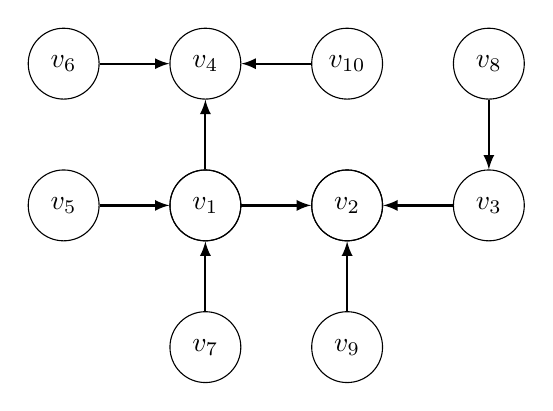
\begin{tikzpicture}
    \draw (-0.9, 0) node[draw = black, circle, minimum size = 
    0.9cm] {};
    \draw (-0.9, 0) node[draw = black, circle, minimum size = 
    0.9cm]
    (v1) {$v_1$};
    \draw (0.9, 0) node[draw = black, circle, minimum size = 
    0.9cm] {};
    \draw (0.9, 0) node[draw = black, circle, minimum size = 0.9cm]
    (v2) {$v_2$};
    \draw (2.7, 0) node[draw = black, circle, minimum size = 0.9cm]
    (v3) {$v_3$};
    \draw (-0.9, 1.8) node[draw = black, circle, minimum size = 0.9cm]
    (v4) {$v_4$};
    \draw (-2.7, 0) node[draw = black, circle, minimum size = 0.9cm]
    (v5) {$v_5$};
    \draw (-2.7, 1.8) node[draw = black, circle, minimum size = 0.9cm]
    (v6) {$v_6$};
    \draw (-0.9, -1.8) node[draw = black, circle, minimum size = 0.9cm]
    (v7) {$v_7$};
    \draw (2.7, 1.8) node[draw = black, circle, minimum size = 0.9cm]
    (v8) {$v_8$};
    \draw (0.9, -1.8) node[draw = black, circle, minimum size = 0.9cm]
    (v9) {$v_9$};
    \draw (0.9, 1.8) node[draw = black, circle, minimum size = 0.9cm]
    (v10) {$v_{10}$};
    \draw[-latex, thick] (v1) -- (v2);
    \draw[-latex, thick] (v3) -- (v2);
    \draw[-latex, thick] (v1) -- (v4);
    \draw[-latex, thick] (v5) -- (v1);
    \draw[-latex, thick] (v6) -- (v4);
    \draw[-latex, thick] (v7) -- (v1);
    \draw[-latex, thick] (v8) -- (v3);
    \draw[-latex, thick] (v9) -- (v2);
    \draw[-latex, thick] (v10) -- (v4);
  \end{tikzpicture}
  \caption{A simple network.}
  \label{fig:network_only}
\end{figure}


\section{Discussion}
\label{sec:discussion}


To be added.




\bibliographystyle{chicago}
\bibliography{citations.bib}


\end{document}
